\documentclass[conference]{IEEEtran} % Usa la classe IEEEtran per formattazione simile

\usepackage{amsmath}
\usepackage{graphicx}



\begin{document}

\title{Exploring the Adversarial Robustness of AI-generated Image Detectors}

\author{
    \IEEEauthorblockN{Thomas Lazzerini, Samuele Cappelletti, Martina D'Angelo}
    \IEEEauthorblockA{
        University of Trento
    }
}

\maketitle

\begin{abstract}
Semi-supervised image classification is a machine-learning task in which a model is trained using a combination of labeled and unlabeled data. This paper consists of a high-level survey of semi-supervised image classification literature and expands on its main theoretical and practical challenges, providing a taxonomy of the most popular semi-supervised learning algorithms. ciao come va
\end{abstract}

\section{Introduction}
Semi-supervised image classification is nowadays a hot research topic. The objective is to tackle the major issue of Supervised Learning: the scarcity of labeled data...
% Continua con il tuo contenuto

As discussed in \cite{zhu2005semi}, semi-supervised learning is an important area of research.

\begin{figure}[h]
    \centering
    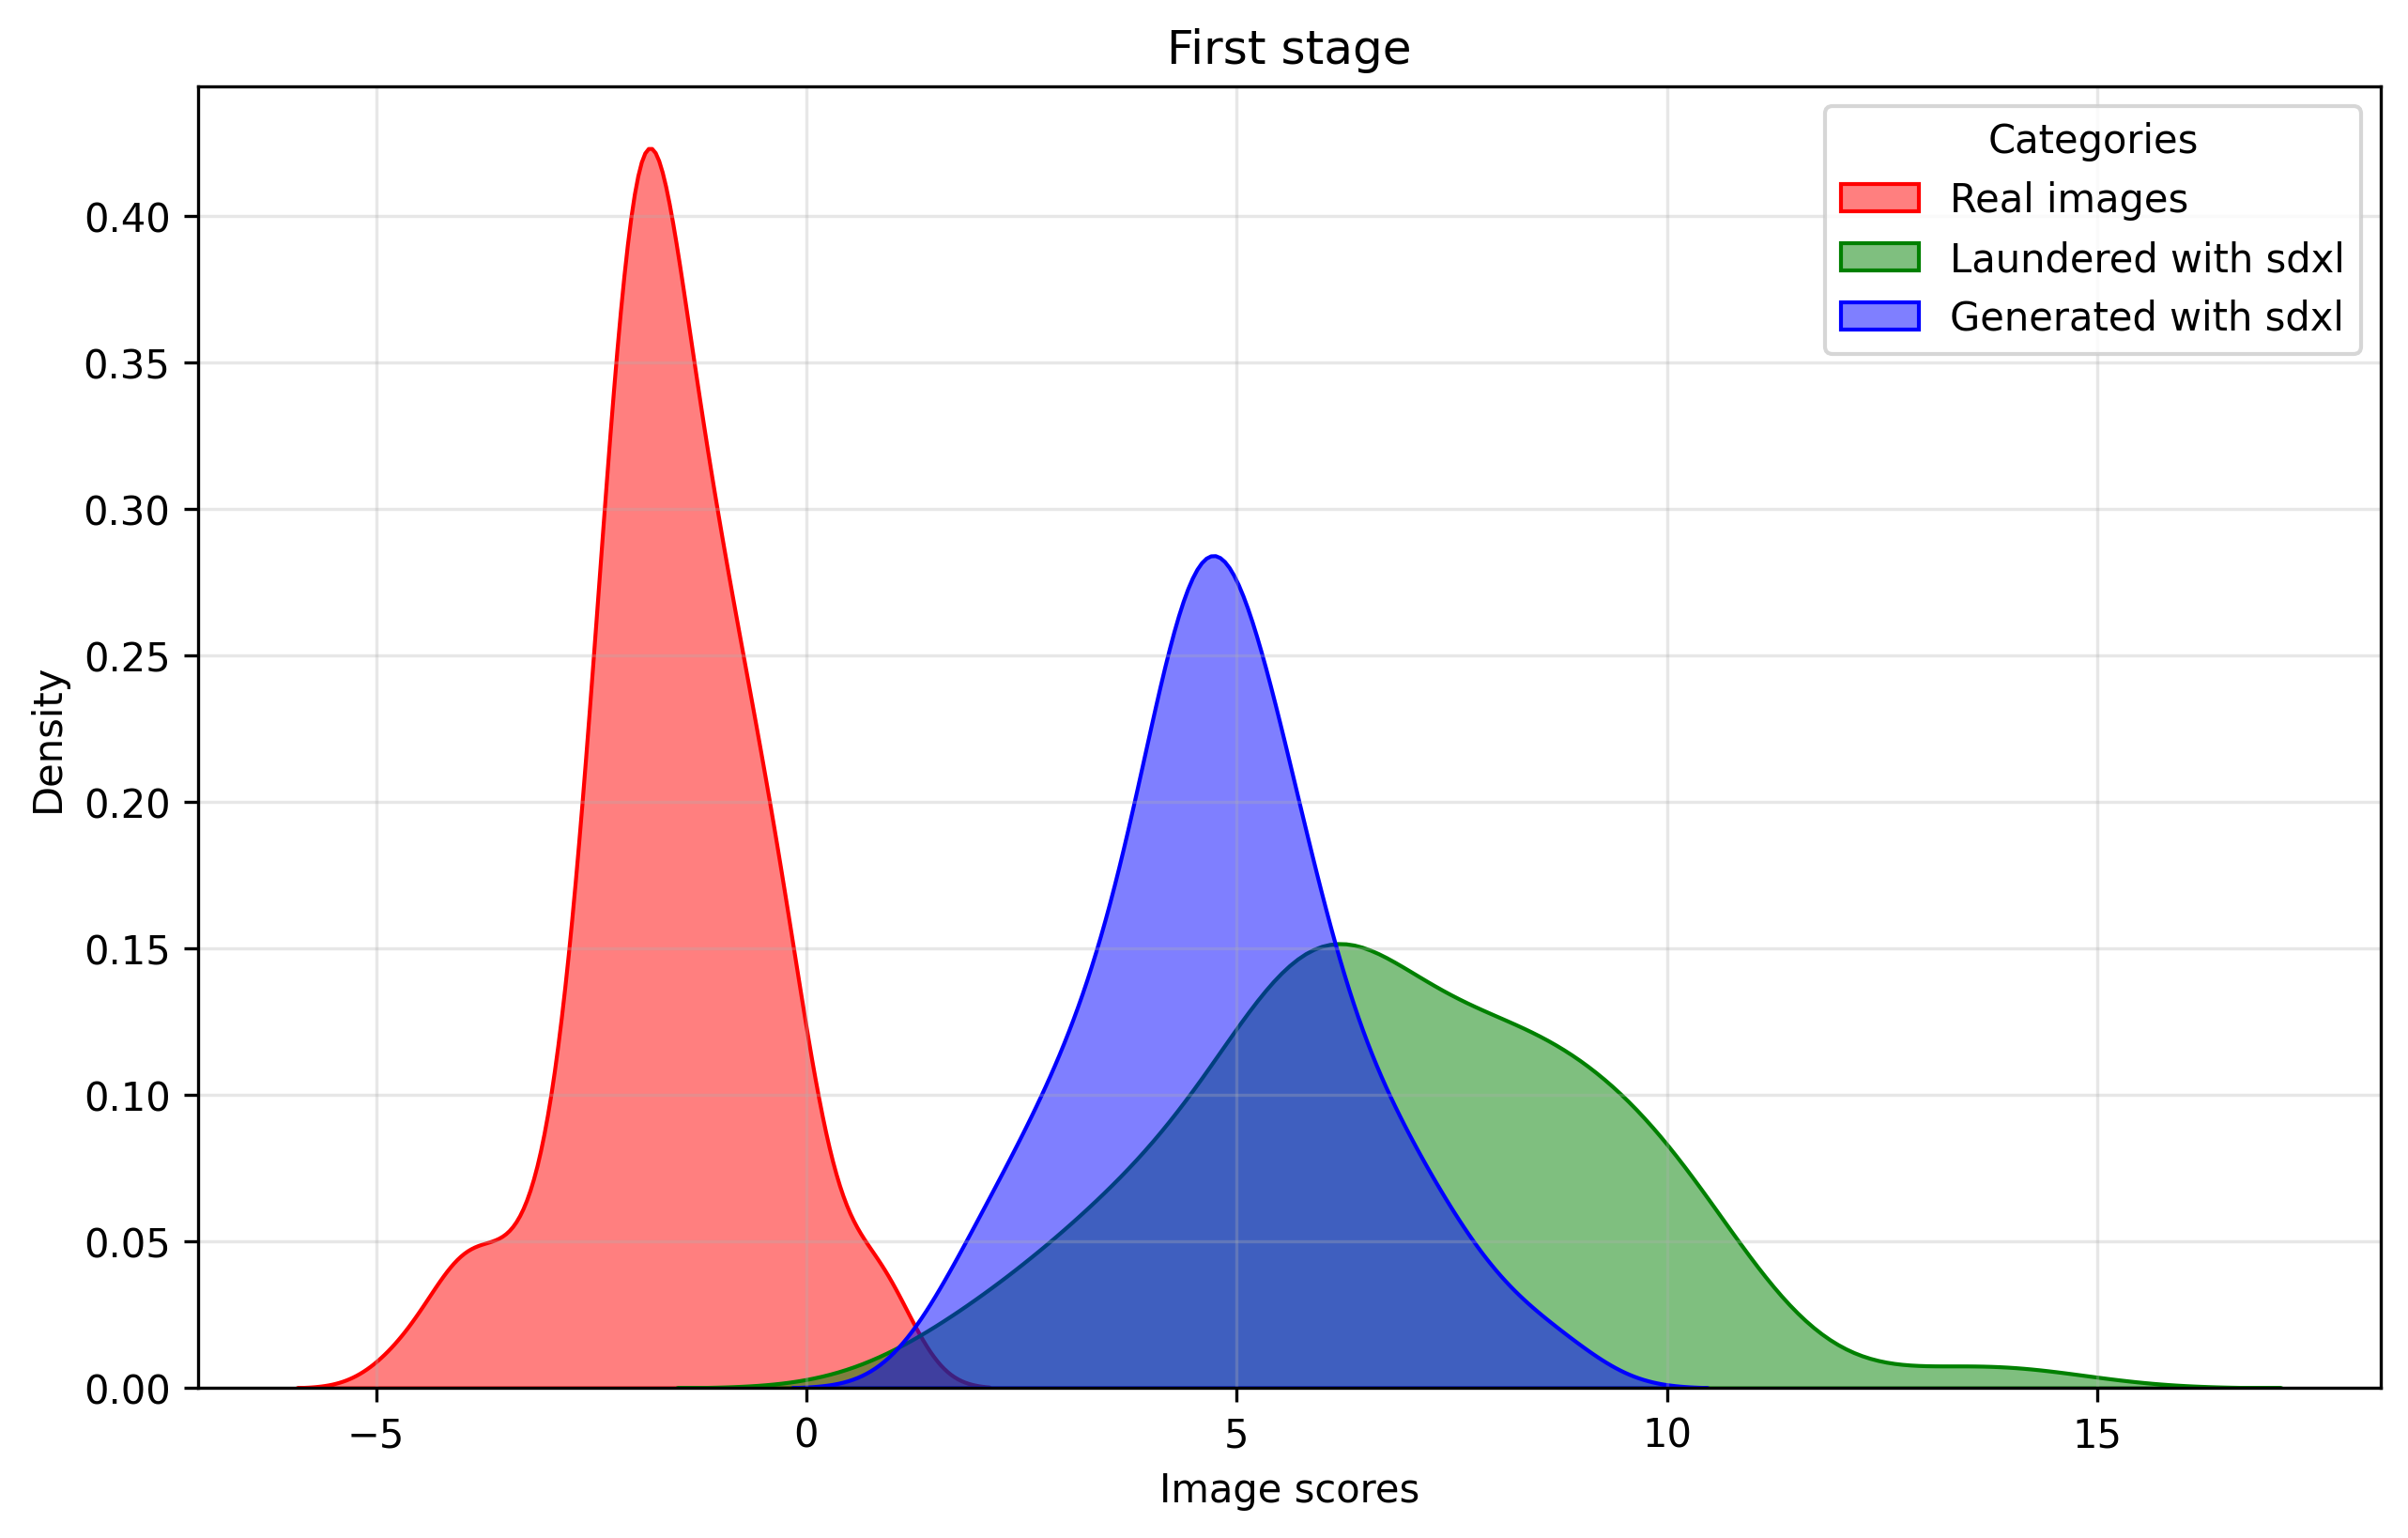
\includegraphics[width=0.8\linewidth]{Img/First_stage.png}
    \caption{Esempio di immagine.}
    \label{fig:esempio}
\end{figure}


\section{Detectors}
    \subsection{CLIP}
    \subsection{PIZZA}
\section{Attacks}
    \subsection{Mimicry}
    \subsection{SD Laundering}
    \subsection{White Black}
    \subsection{Adversarial Robustness}
\section{Experiment}
\section{Conclusions}


% =====================================================================================
\section(White Black)

Evaluating deepfake-image detectors reveals their vulnerabilities to both white- and black-box attacks, significantly reducing their effectiveness. For instance, powerful forensic classifiers can be compromised to achieve near 0\% accuracy under various attack scenarios. A state-of-the-art classifier, as demonstrated by Wang et al. \cite{Wang_2020_CVPR}, achieves an area under the ROC curve (AUC) of 0.95 when trained on a single generator, yet remains susceptible to adversarial perturbations \cite{mardeenpaper1}.
The attacks are categorized into two conditions:
\begin{itemize}
    \item White-box attacks, where full access to the classifier's parameters is available.
    \item Black-box attacks, where only the classifier type is known, utilizing adversarial examples that transfer misclassifications across models
\end{itemize}

They introduce four attack types targeting the classifier from Wang et al. \cite{Wang_2020_CVPR}:
\begin{itemize}
    \item Image-specific attacks: These modify input images with perturbations to deceive detectors (eg. PGD, DI2-FGSM)
    \begin{itemize}
    \item Loss-Maximizing Attack: this attack maximizes the likelihood that a fake image $x$ perturbed by $\delta$ is misclassified as real. This attack was found to be highly effective and even with flipping the lowest-order bit of 40\% of pixels for uncompressed images, the AUC reduces from 0.966 to 0.27.
    \end{itemize}
    \item Universal Attacks: These create a single adversarial perturbation applicable across various images, reducing computational costs.
    \begin{itemize}
        \item  Universal Adversarial-Patch Attack: A universal patch overlaid on images reduces AUC from 0.966 to 0.085.
        \item Universal Latent-Space Attack: Instead of altering images directly, this method modifies low-level attributes of the generative model, resulting in an AUC drop from 0.99 to 0.17.
    \end{itemize} 
    \item Black-Box Transfer Attack: This approach uses adversarial examples from a surrogate model to impair a more robust classifier's performance. By transferring adversarial examples they develop their own forensic classifier and trasfer the attack to the target classifier \cite{Wang_2020_CVPR}, the AUC is reduced from 0.96 to 0.22. 
\end{itemize}

Insights into attack transferability \cite{mardeenpaper2} reveal that attacks effective on one model often struggle against others. Transferability is notably successful within the same family of detectors, such as CNN to CNN or CLIP to CLIP, but less so between different families (e.g., CNN and CLIP). While both CNN and CLIP models are vulnerable to white-box attacks, CLIP models demonstrate greater robustness, particularly against fake-to-real attacks.
The low transferability of adversarial attacks suggests that distinct model architectures process images differently:
CNN-based detectors focus on medium-to-high frequencies and isotropic spectra, while CLIP-based detectors rely on low-frequency patterns and cross-shaped spectra.
This architectural divergence contributes to the limited effectiveness of attacks across model types, indicating that successful defenses must consider these fundamental differences in image processing.

The forger holds a strategic advantage, needing to devise only one successful attack, while the defender must guard against all potential threats. Notably, detectors trained on ImageNet \cite{denglarge} are particularly vulnerable; forensic classifiers require perturbations approximately ten times smaller than those needed to deceive ImageNet classifiers, possibly due to JPEG artifacts present in the training data \cite{mardeenpaper1}.
Two effective defenses have emerged:
\begin{itemize}
    \item Adversarial Training: This technique involves continuously training the classifier on adversarial examples generated from previous iterations, enhancing its robustness.
    \item Randomized Smoothing: This method adds significant Gaussian noise to each pixel, making it provably impossible for small perturbations to alter the classifier's output.
\end{itemize}

Forensic classifiers must integrate an adversarial model into their defenses that extends beyond standard techniques like recompression, resizing, blurring, or adding white noise. This comprehensive approach is essential for improving resilience against increasingly sophisticated attacks.

%%%%%%%%%%%%%%%%%%%%%% ======================== END

\bibliographystyle{IEEEtran} % Stile delle referenze (es. IEEE)
\bibliography{references}    % Nome del file .bib (senza estensione)

\end{document}